\subsection*{Producto mínimo viable}
\addcontentsline{toc}{subsection}{Producto mínimo viable}

El Producto Mínimo Viable (MVP) corresponde a una versión inicial del producto que contiene únicamente las funcionalidades esenciales necesarias para satisfacer a los primeros usuarios y validar las hipótesis fundamentales del modelo de negocio. Su objetivo principal es poner el producto en manos de los usuarios lo más pronto posible, permitiendo recopilar retroalimentación real que facilite iteraciones y mejoras posteriores \parencite{IntuitChamp01}.

A partir de un punto de vista técnico, definir el Producto Mínimo Viable no es solamente seleccionar funcionalidades básicas del sistema sino también en establecer una arquitectura tecnológica el cual permita desarrollar, probar y evolucionar dichas funcionalidades de forma eficiente. En este contexto, el diseño del sistema se plantea desde la formulación de una arquitectura y el despliegue del sistema.

Cabe aclarar que la arquitectura del sistema y su modelo de despliegue son dos cosas diferentes, por un lado la arquitectura define la estructura lógica y el comportamiento de los diferentes servicios entre sí, mientras que el despliegue es la vía por la cual estos componentes se organizan e implementan dentro de la infraestructura tecnológica \parencite{BBVA04}.

A continuación se describirán las tecnologías usadas y los motivos por los cuales fueron seleccionados para el progreso del proyecto:

\subsection*{Arquitectura del Sistema}
\addcontentsline{toc}{subsection}{Arquitectura del Sistema}

Para el desarrollo de la plataforma, se propone una \textbf{Arquitectura de Microservicios} basada en la nube, la cual permite desacoplar las funcionalidades críticas del sistema para garantizar escalabilidad, mantenibilidad y alta disponibilidad. Esta estructura es ideal para un ecosistema digital que integra procesamiento de datos financieros y algoritmos de aprendizaje automático, facilitando la actualización independiente de cada componente sin afectar la integridad global del servicio.

Los componentes principales de la arquitectura se dividen en las siguientes capas:

\begin{itemize}
	\item \textbf{Capa de Presentación (Frontend):} Desarrollada bajo un enfoque de aplicación web progresiva (PWA), permitiendo el acceso multiplataforma. Se centra en la entrega de interfaces didácticas y simuladores interactivos con una experiencia de usuario (UX) optimizada para dispositivos móviles.
	
	\item \textbf{Capa de Lógica de Negocio (Backend):} Compuesta por microservicios independientes que gestionan la autenticación de usuarios, la lógica de los simuladores financieros y la administración de módulos educativos. 
	
	\item \textbf{Capa de Inteligencia Artificial (AI Service):} Un servicio especializado dedicado al entrenamiento y ejecución de modelos de \textit{Machine Learning}. Este componente consume datos de comportamiento del usuario para generar recomendaciones personalizadas y proyecciones financieras adaptativas \parencite{BBVAResearch01}.
	
	\item \textbf{Capa de Datos:} Implementación de una base de datos híbrida que utiliza sistemas relacionales (PostgreSQL) para la gestión de transacciones y perfiles de usuario, junto con almacenes de datos no relacionales (NoSQL) para el procesamiento de grandes volúmenes de eventos y telemetría de aprendizaje.
\end{itemize}

\subsubsection*{Justificación Técnica de la Arquitectura}
\addcontentsline{toc}{subsubsection}{Justificación Técnica de la Arquitectura}
La elección de microservicios sobre una arquitectura monolítica responde a la naturaleza del emprendimiento bajo la metodología \textit{Lean Startup}. Esta arquitectura permite:
\begin{enumerate}
	\item \textbf{Escalabilidad Adaptativa:} Capacidad de aumentar los recursos del microservicio de IA durante picos de demanda sin necesidad de replicar todo el sistema.
	\item \textbf{Resiliencia:} Si el módulo de recomendaciones experimenta una falla, las herramientas básicas de simulación y el contenido educativo permanecen operativos para el usuario.
	\item \textbf{Integración Continua:} Facilita el despliegue de actualizaciones rápidas basadas en la retroalimentación del mercado en Bogotá, permitiendo pivotar funcionalidades técnicas de manera ágil.
\end{enumerate}

\subsubsection*{Modelado de la Infraestructura y Componentes}
\addcontentsline{toc}{subsubsection}{Modelado de la Infraestructura y Componentes}
A continuación, se describen los diagramas técnicos que representan la organización lógica y la distribución física de la plataforma.

\paragraph*{Diagrama de Arquitectura Lógica}
\addcontentsline{toc}{paragraph}{Diagrama de Arquitectura Lógica}
Este diagrama ilustra la interacción entre los distintos servicios a través de un \textit{API Gateway}, que actúa como punto de entrada único para las solicitudes de los usuarios.

\begin{itemize}
	\item \textbf{API Gateway:} Gestiona el enrutamiento, la autenticación mediante \textit{JSON Web Tokens} (JWT) y el balanceo de carga.
	\item \textbf{Microservicios Centrales:} Servicios aislados para el manejo de la lógica educativa y los simuladores financieros.
	\item \textbf{ML Engine:} Microservicio independiente en Python que ejecuta los algoritmos de recomendación.
	\item \textbf{Message Broker:} Facilita la comunicación asíncrona entre servicios para procesos de fondo, como el envío de reportes financieros.
\end{itemize}

\paragraph*{Diagrama de Despliegue}
\addcontentsline{toc}{paragraph}{Diagrama de Despliegue}
El diagrama de despliegue detalla la disposición física de los componentes en la infraestructura de nube. Se utiliza una estrategia de \textbf{Contenerización} con Docker, orquestada para asegurar que el sistema sea agnóstico respecto al proveedor de nube (AWS, Azure o Google Cloud).


\begin{itemize}
	\item \textbf{Cliente:} Representa el nodo del dispositivo del usuario (móvil o escritorio) que se comunica vía HTTPS.
	\item \textbf{Cloud Cluster:} Nodo principal donde residen los contenedores de los microservicios.
	\item \textbf{Data Tier:} Instancias de base de datos administradas que garantizan la persistencia y copias de seguridad automáticas de la información financiera de los usuarios.
	\item \textbf{CDN (Content Delivery Network):} Nodo encargado de distribuir el contenido multimedia de aprendizaje de manera eficiente en la región de Bogotá.
\end{itemize}

\begin{figure}[H]
	\centering
	% \includegraphics[width=0.8\textwidth]{Imagenes/DiagramaArquitectura.png}
	\caption{Arquitectura Lógica de Microservicios de la Plataforma.}
	\label{fig:arquitectura_logica}
\end{figure}

\begin{figure}[H]
	\centering
	% \includegraphics[width=0.8\textwidth]{Imagenes/DiagramaDespliegue.png}
	\caption{Diagrama de Despliegue de Infraestructura en la Nube.}
	\label{fig:despliegue_fisico}
\end{figure}

\subsubsection*{Tecnologías}
\addcontentsline{toc}{subsubsection}{Tecnologías}

Para garantizar la viabilidad técnica del Producto Mínimo Viable y soportar la arquitectura de microservicios propuesta, se han seleccionado tecnologías que priorizan el rendimiento, la escalabilidad y un entorno de desarrollo moderno.

\begin{itemize}
	\item \textbf{Frontend (Framework):} Se utilizará \textbf{Angular}. Este framework basado en TypeScript proporciona una estructura modular mediante componentes y servicios, facilitando la creación de una interfaz altamente interactiva. Al ser una aplicación de una sola página (SPA), permite transiciones fluidas en los simuladores financieros y una experiencia de usuario (UX) coherente con los estándares actuales de las aplicaciones bancarias.
	
	\item \textbf{Backend (Entorno de ejecución):} Los microservicios de lógica de negocio y el API Gateway se desarrollarán sobre \textbf{Node.js}. Su arquitectura basada en eventos y entrada/salida no bloqueante asegura que la plataforma pueda manejar múltiples peticiones simultáneas, como el procesamiento de datos de entrenamiento para la IA y las consultas de los usuarios a los simuladores.
	
	\item \textbf{Inteligencia Artificial y ML:} Para el procesamiento de datos adaptativo se empleará \textbf{Python}, utilizando librerías como Scikit-learn o TensorFlow. Los modelos de recomendación se expondrán como servicios independientes que interactúan con el backend de Node.js de manera asíncrona.
	
	\item \textbf{Bases de Datos:} 
	\begin{itemize}
		\item \textbf{PostgreSQL:} Motor de base de datos relacional para la gestión de usuarios, seguridad y transacciones, asegurando la integridad referencial de la información financiera.
		\item \textbf{MongoDB / NoSQL:} Para el almacenamiento de contenido educativo dinámico y el registro de eventos de aprendizaje, cuya estructura requiere flexibilidad frente a cambios constantes.
	\end{itemize}
	
	\item \textbf{Infraestructura y Contenerización:} 
	\begin{itemize}
		\item \textbf{Docker:} Se emplearán contenedores para aislar cada servicio (Angular, Node.js y Python), garantizando que el sistema sea agnóstico respecto al sistema operativo de despliegue y facilitando la integración continua.
	\end{itemize}
\end{itemize}

\subsubsection*{Análisis de Integración Tecnológica}
La integración de Node.js y Angular asegura un ecosistema de desarrollo homogéneo bajo JavaScript/TypeScript. Esto reduce la curva de aprendizaje y mejora la velocidad de implementación del PMV, permitiendo que el equipo de desarrollo se enfoque en la optimización de los algoritmos de personalización financiera y en la validación rápida de hipótesis bajo la metodología \textit{Lean Startup}.

\subsubsection*{Requerimientos}
\addcontentsline{toc}{subsubsection}{Requerimientos}
A continuación, se especifican los requerimientos del sistema, los cuales establecen las capacidades funcionales y las restricciones de calidad que debe cumplir la plataforma para satisfacer los objetivos del proyecto.

\paragraph*{Requerimientos funcionales}
\addcontentsline{toc}{paragraph}{Requerimientos funcionales}
Los requerimientos funcionales describen las acciones específicas que debe realizar el sistema, estos requerimientos funcionales se describen a continuación:

\begin{table}[H]
	\begin{tabular}{|a{5cm}|m{11cm}|}
		\hline
		\textbf{Código} & RF01 \\ \hline
		\textbf{Nombre del requerimiento} & Registro de cuenta de usuarios \\ \hline
		\textbf{Fecha} & 15/10/2025 \\ \hline
		\textbf{Tipo de requerimiento} & Funcional \\ \hline
		\textbf{Origen de requerimiento} & Análisis del sistema \\ \hline
		\textbf{Prioridad} & Alta \\ \hline
		\textbf{Actor} & Usuario y administrador \\ \hline
		\textbf{Descripción} & El sistema debe permitir a los nuevos usuarios crear una cuenta mediante un formulario que capture nombre completo, correo electrónico y contraseña. El sistema debe validar que el correo no esté registrado previamente y cifrar la contraseña antes de almacenarla.\\ \hline
		\textbf{Criterio de aceptación} & Se crea un nuevo registro en la base de datos PostgreSQL y el sistema redirige al usuario al flujo de bienvenida o verificación de correo.. \\ \hline
	\end{tabular}
\end{table}

\begin{table}[H]
	\begin{tabular}{|a{5cm}|m{11cm}|}
		\hline
		\textbf{Código} & RF02 \\ \hline
		\textbf{Nombre del requerimiento} & Autenticación y Control de Acceso \\ \hline
		\textbf{Fecha} & 15/10/2025 \\ \hline
		\textbf{Tipo de requerimiento} & Funcional \\ \hline
		\textbf{Origen de requerimiento} & Análisis del sistema \\ \hline
		\textbf{Prioridad} & Alta \\ \hline
		\textbf{Actor} & Usuario y administrador \\ \hline
		\textbf{Descripción} & El sistema debe validar las credenciales del usuario (email y contraseña) contra los registros existentes. Tras una validación exitosa, el backend debe generar un token de acceso (JWT) que permita al usuario consumir los servicios protegidos de la arquitectura de microservicios. \\ \hline
		\textbf{Criterio de aceptación} & El usuario accede a su sesión privada; en caso de credenciales inválidas, el sistema debe denegar el acceso y mostrar un mensaje de error genérico por seguridad. \\ \hline
	\end{tabular}
\end{table}

\begin{table}[H]
	\begin{tabular}{|a{5cm}|m{11cm}|}
		\hline
		\textbf{Código} & RF03 \\ \hline
		\textbf{Nombre del requerimiento} & Gestión y Caracterización de Perfil de Usuario \\ \hline
		\textbf{Fecha} & 15/10/2025 \\ \hline
		\textbf{Tipo de requerimiento} & Funcional \\ \hline
		\textbf{Origen de requerimiento} & Análisis del sistema \\ \hline
		\textbf{Prioridad} & Media \\ \hline
		\textbf{Actor} & Usuario y sistema \\ \hline
		\textbf{Descripción} & El sistema debe permitir al usuario completar y actualizar su información sociodemográfica y financiera básica (ingresos, metas, tipo de ocupación). Estos datos deben persistir para alimentar de forma dinámica el motor de recomendaciones. \\ \hline
		\textbf{Criterio de aceptación} & El perfil se guarda correctamente en PostgreSQL; los cambios se reflejan inmediatamente en la interfaz y quedan disponibles para el microservicio de Machine Learning. \\ \hline
	\end{tabular}
\end{table}

\begin{table}[H]
	\begin{tabular}{|a{5cm}|m{11cm}|}
		\hline
		\textbf{Código} & RF04 \\ \hline
		\textbf{Nombre del requerimiento} & Motor de Simulaciones Financieras Adaptativas \\ \hline
		\textbf{Fecha} & 15/10/2025 \\ \hline
		\textbf{Tipo de requerimiento} & Funcional \\ \hline
		\textbf{Origen de requerimiento} & Plan de negocio \\ \hline
		\textbf{Prioridad} & Alta \\ \hline
		\textbf{Actor} & Usuario \\ \hline
		\textbf{Descripción} & El sistema debe proveer herramientas de cálculo para ahorro, crédito e inversión. Debe procesar variables de entrada (capital, tiempo, tasa) y devolver proyecciones basadas en modelos financieros estandarizados. \\ \hline
		\textbf{Criterio de aceptación} & El motor de cálculo devuelve resultados con precisión decimal; los datos se visualizan mediante componentes gráficos interactivos en Angular. \\ \hline
	\end{tabular}
\end{table}


\begin{table}[H]
	\begin{tabular}{|a{5cm}|m{11cm}|}
		\hline
		\textbf{Código} & RF05 \\ \hline
		\textbf{Nombre del requerimiento} & Gestión de presupuesto y ahorro \\ \hline
		\textbf{Fecha} & 15/10/2025 \\ \hline
		\textbf{Tipo de requerimiento} & Funcional \\ \hline
		\textbf{Origen de requerimiento} & Estudio de usabilidad \\ \hline
		\textbf{Prioridad} & Media \\ \hline
		\textbf{Actor} & Usuario \\ \hline
		\textbf{Descripción} & Módulo para registrar ingresos y gastos con interfaz intuitiva e incentivos (puntos o insignias) al alcanzar metas de ahorro. \\ \hline
		\textbf{Criterio de aceptación} & El usuario añade o clasifica transacciones; la app actualiza totales y gráficos de presupuesto, y otorga recompensas al lograr metas definidas (ver perfil con puntos/insignias). \\ \hline
	\end{tabular}
\end{table}

\begin{table}[H]
	\begin{tabular}{|a{5cm}|m{11cm}|}
		\hline
		\textbf{Código} & RF06 \\ \hline
		\textbf{Nombre del requerimiento} & Servicio Automatizado de Notificaciones \\ \hline
		\textbf{Fecha} & 15/10/2025 \\ \hline
		\textbf{Tipo de requerimiento} & Funcional \\ \hline
		\textbf{Origen de requerimiento} & Análisis del sistema \\ \hline
		\textbf{Prioridad} & Media \\ \hline
		\textbf{Actor} & Usuario y sistema \\ \hline
		\textbf{Descripción} & El sistema debe programar y enviar alertas automáticas basadas en fechas de vencimiento de obligaciones financieras o proximidad al cumplimiento de metas de ahorro definidas por el usuario. \\ \hline
		\textbf{Criterio de aceptación} & El microservicio de notificaciones dispara la alerta en la fecha y hora configurada; el usuario recibe la notificación de manera asíncrona en la plataforma. \\ \hline
	\end{tabular}
\end{table}

\begin{table}[H]
	\begin{tabular}{|a{5cm}|m{11cm}|}
		\hline
		\textbf{Código} & RF07 \\ \hline
		\textbf{Nombre del requerimiento} & Adquisición de plan de suscripción \\ \hline
		\textbf{Fecha} & 15/10/2025 \\ \hline
		\textbf{Tipo de requerimiento} & Funcional \\ \hline
		\textbf{Origen de requerimiento} & Comercialización \\ \hline
		\textbf{Prioridad} & Alta \\ \hline
		\textbf{Actor} & Usuario \\ \hline
		\textbf{Descripción} & El sistema debe ofrecer al usuario la posiblidad de seleccionar y suscribirse a la plataforma, ofreciendo un mayor número de características y menores límites. \\ \hline
		\textbf{Criterio de aceptación} & El usuario puede seleccionar y adquirir la suscripción directamente desde el sistema, con un proceso de pago en línea exitoso y confirmando la suscripción. \\ \hline
	\end{tabular}
\end{table}

\begin{table}[H]
	\begin{tabular}{|a{5cm}|m{11cm}|}
		\hline
		\textbf{Código} & RF08 \\ \hline
		\textbf{Nombre del requerimiento} & Motor de Personalización (Machine Learning) \\ \hline
		\textbf{Fecha} & 15/10/2025 \\ \hline
		\textbf{Tipo de requerimiento} & Funcional \\ \hline
		\textbf{Origen de requerimiento} & Plan de negocio \\ \hline
		\textbf{Prioridad} & Alta \\ \hline
		\textbf{Actor} & Usuario y sistema\\ \hline
		\textbf{Descripción} & Implementación de un microservicio en Python que analice el perfil del usuario y sugiera una ruta de aprendizaje personalizada (módulos educativos y metas de ahorro). \\ \hline
		\textbf{Criterio de aceptación} & El sistema debe generar al menos tres recomendaciones de contenido basadas en los datos de entrada del usuario con una latencia de respuesta inferior a 2 segundos. \\ \hline
	\end{tabular}
\end{table}

\begin{table}[H]
	\begin{tabular}{|a{5cm}|m{11cm}|}
		\hline
		\textbf{Código} & RF09 \\ \hline
		\textbf{Nombre del requerimiento} & Visualización y Consumo de Módulos Educativos \\ \hline
		\textbf{Fecha} & 15/10/2025 \\ \hline
		\textbf{Tipo de requerimiento} & Funcional \\ \hline
		\textbf{Origen de requerimiento} & Plan de negocio \\ \hline
		\textbf{Prioridad} & Alta \\ \hline
		\textbf{Actor} & Usuario \\ \hline
		\textbf{Descripción} & El sistema debe presentar los módulos de aprendizaje financiero (texto, video, cuestionarios) organizados por categorías o según la ruta personalizada generada por la IA. \\ \hline
		\textbf{Criterio de aceptación} & El usuario puede acceder al contenido, marcar módulos como completados y visualizar su progreso en la barra de avance de la plataforma. \\ \hline
	\end{tabular}
\end{table}

\begin{table}[H]
	\begin{tabular}{|a{5cm}|m{11cm}|}
		\hline
		\textbf{Código} & RF10 \\ \hline
		\textbf{Nombre del requerimiento} & Panel de Administración de Contenidos y Usuarios \\ \hline
		\textbf{Fecha} & 15/10/2025 \\ \hline
		\textbf{Tipo de requerimiento} & Funcional \\ \hline
		\textbf{Origen de requerimiento} & Análisis del sistema \\ \hline
		\textbf{Prioridad} & Media \\ \hline
		\textbf{Actor} & Administrador \\ \hline
		\textbf{Descripción} & El sistema debe proveer una interfaz para que el administrador gestione usuarios, actualice las tasas de interés de referencia para los simuladores y cargue nuevo material educativo. \\ \hline
		\textbf{Criterio de aceptación} & Las actualizaciones realizadas en el panel se reflejan en la base de datos y afectan globalmente el comportamiento de los simuladores y módulos educativos. \\ \hline
	\end{tabular}
\end{table}

\begin{table}[H]
	\begin{tabular}{|a{5cm}|m{11cm}|}
		\hline
		\textbf{Código} & RF11 \\ \hline
		\textbf{Nombre del requerimiento} & Finalización de Sesión (Logout) \\ \hline
		\textbf{Fecha} & 15/10/2025 \\ \hline
		\textbf{Tipo de requerimiento} & Funcional \\ \hline
		\textbf{Origen de requerimiento} & Análisis del sistema \\ \hline
		\textbf{Prioridad} & Alta \\ \hline
		\textbf{Actor} & Usuario y Administrador \\ \hline
		\textbf{Descripción} & El sistema debe permitir el cierre de sesión voluntario, invalidando el token JWT en el cliente y redirigiendo al usuario a la interfaz pública de la plataforma. \\ \hline
		\textbf{Criterio de aceptación} & El token se elimina del almacenamiento local; cualquier intento posterior de acceder a rutas protegidas (/dashboard, /perfil) es rechazado por el sistema. \\ \hline
	\end{tabular}
\end{table}

%Pendiente por revisar requerimientos no funcionales y casos de uso%

\paragraph*{Requerimientos no funcionales}
\addcontentsline{toc}{paragraph}{Requerimientos no funcionales}
Los requerimientos no funcionales describen las cualidades y estándares que debe tener el sistema, su comportamiento, y otros aspectos. Estos requerimientos no funcionales se describen a continuación:

\begin{table}[H]
	\begin{tabular}{|s{5cm}|m{11cm}|}
		\hline
		\textbf{Código} & RNF01 \\ \hline
		\textbf{Nombre del requerimiento} & Compatibilidad web \\ \hline
		\textbf{Fecha} & 15/10/2025 \\ \hline
		\textbf{Tipo de requerimiento} & No funcional \\ \hline
		\textbf{Origen de requerimiento} & Tendencias tecnológicas \\ \hline
		\textbf{Prioridad} & Alta \\ \hline
		\textbf{Descripción} & Aplicación nativa o multiplataforma para dispositivos de computadora, optimizada para distintos tamaños de pantalla. \\ \hline
		\textbf{Criterio de aceptación} & Se ejecuta en buscadores web; la interfaz se adapta correctamente sin elementos desalineados. \\ \hline
	\end{tabular}
\end{table}

\begin{table}[H]
	\begin{tabular}{|s{5cm}|m{11cm}|}
		\hline
		\textbf{Código} & RNF02 \\ \hline
		\textbf{Nombre del requerimiento} & Interfaz intuitiva y amigable \\ \hline
		\textbf{Fecha} & 15/10/2025 \\ \hline
		\textbf{Tipo de requerimiento} & No funcional \\ \hline
		\textbf{Origen de requerimiento} & Estudio de usabilidad \\ \hline
		\textbf{Prioridad} & Alta \\ \hline
		\textbf{Descripción} & Aplicación web optimizada para distintos tamaños de pantalla. \\ \hline
		\textbf{Criterio de aceptación} & En pruebas de usuario, al menos el 80\% completa tareas básicas (registro, simulación) sin asistencia. La interfaz es valorada como fácil de usar en encuestas. \\ \hline
	\end{tabular}
\end{table}

\begin{table}[H]
	\begin{tabular}{|s{5cm}|m{11cm}|}
		\hline
		\textbf{Código} & RNF03 \\ \hline
		\textbf{Nombre del requerimiento} & Acceso a funcionalidades por rol \\ \hline
		\textbf{Fecha} & 15/10/2025 \\ \hline
		\textbf{Tipo de requerimiento} & No funcional \\ \hline
		\textbf{Origen de requerimiento} & Gestión de usuarios \\ \hline
		\textbf{Prioridad} & Alta \\ \hline
		\textbf{Descripción} & El sistema deberá permitir el acceso a diferentes funcionalidades dependiendo del rol que tenga el usuario (administrador, plan pagado o plan gratuito). Además cada rol debe tener permisos en específico que limiten o amplien el acceso a ciertas secciones o funciones dentro de la plataforma. \\ \hline
		\textbf{Criterio de aceptación} & Las personas que ingresen a nuestra plataforma tendrán su rol correctamente al iniciar sesión con sus cuentas. \\ \hline
	\end{tabular}
\end{table}

\begin{table}[H]
	\begin{tabular}{|s{5cm}|m{11cm}|}
		\hline
		\textbf{Código} & RNF04 \\ \hline
		\textbf{Nombre del requerimiento} & Seguridad de la información \\ \hline
		\textbf{Fecha} & 15/10/2025 \\ \hline
		\textbf{Tipo de requerimiento} & No funcional \\ \hline
		\textbf{Origen de requerimiento} & Normativa legal de seguridad \\ \hline
		\textbf{Prioridad} & Alta \\ \hline
		\textbf{Descripción} & Protección de datos personales y financieros: cifrado en tránsito (HTTPS/TLS) y reposo; autenticación segura (idealmente 2FA opcional). \\ \hline
		\textbf{Criterio de aceptación} & El sistema utiliza protocolos de cifrado estándar (TLS 1.2+); las contraseñas están encriptadas. En pruebas de penetración, no se obtienen datos sensibles. \\ \hline
	\end{tabular}
\end{table}

\begin{table}[H]
	\begin{tabular}{|s{5cm}|m{11cm}|}
		\hline
		\textbf{Código} & RNF05 \\ \hline
		\textbf{Nombre del requerimiento} & Privacidad del usuario \\ \hline
		\textbf{Fecha} & 15/10/2025 \\ \hline
		\textbf{Tipo de requerimiento} & No funcional \\ \hline
		\textbf{Origen de requerimiento} & Legislación de protección de datos \\ \hline
		\textbf{Prioridad} & Alta \\ \hline
		\textbf{Descripción} & Cumplimiento de leyes colombianas de datos (ej. Ley 1581/2012): obtener consentimiento informado antes de recolectar datos. \\ \hline
		\textbf{Criterio de aceptación} & El usuario acepta política de privacidad al registrarse; la app no comparte datos sin permiso. Se verifica que exista consentimiento explícito. \\ \hline
	\end{tabular}
\end{table}

\begin{table}[H]
	\begin{tabular}{|s{5cm}|m{11cm}|}
		\hline
		\textbf{Código} & RNF06 \\ \hline
		\textbf{Nombre del requerimiento} & Rendimiento \\ \hline
		\textbf{Fecha} & 15/10/2025 \\ \hline
		\textbf{Tipo de requerimiento} & No funcional \\ \hline
		\textbf{Origen de requerimiento} & Experiencia de usuario \\ \hline
		\textbf{Prioridad} & Media \\ \hline
		\textbf{Descripción} & Operaciones clave (simulaciones, navegación) deben responder rápido (p.ej. <5 segundos), incluso con datos moderados. \\ \hline
		\textbf{Criterio de aceptación} & Mediciones de rendimiento indican tiempo de respuesta promedio < 5s bajo carga normal. El inicio de la app carga en menos de 3,5s en dispositivo estándar. \\ \hline
	\end{tabular}
\end{table}

\begin{table}[H]
	\begin{tabular}{|s{5cm}|m{11cm}|}
		\hline
		\textbf{Código} & RNF07 \\ \hline
		\textbf{Nombre del requerimiento} & Disponibilidad y confiabilidad \\ \hline
		\textbf{Fecha} & 15/10/2025 \\ \hline
		\textbf{Tipo de requerimiento} & No funcional \\ \hline
		\textbf{Origen de requerimiento} & Acuerdo de Nivel de Servicio (SLA) \\ \hline
		\textbf{Prioridad} & Media \\ \hline
		\textbf{Descripción} & Sistema con alta disponibilidad (por ejemplo, 95\% de uptime mensual) y respaldos periódicos automáticos de los datos, incluidos perfiles y planes adquiridos. \\ \hline
		\textbf{Criterio de aceptación} & Registros de sistema muestran al menos un 95\% de uptime. Al simular una interrupción, el servicio se restablece automáticamente o en menos de 1 hora según lo establecido, además de tener una copia de seguridad con los datos almacenados. \\ \hline
	\end{tabular}
\end{table}

\begin{table}[H]
	\begin{tabular}{|s{5cm}|m{11cm}|}
		\hline
		\textbf{Código} & RNF08 \\ \hline
		\textbf{Nombre del requerimiento} & Accesibilidad \\ \hline
		\textbf{Fecha} & 15/10/2025 \\ \hline
		\textbf{Tipo de requerimiento} & No funcional \\ \hline
		\textbf{Origen de requerimiento} & Requerimientos de accesibilidad \\ \hline
		\textbf{Prioridad} & Media \\ \hline
		\textbf{Descripción} & Cumplir estándares básicos (p.ej. WCAG 2.1 AA): contraste adecuado, etiquetas en controles, navegación compatible con lectores de pantalla. \\ \hline
		\textbf{Criterio de aceptación} & Verificación WCAG: textos legibles y contrastados, elementos interactivos etiquetados. Se confirma funcionalidad con un lector de pantalla. \\ \hline
	\end{tabular}
\end{table}

\begin{table}[H]
	\begin{tabular}{|s{5cm}|m{11cm}|}
		\hline
		\textbf{Código} & RNF09 \\ \hline
		\textbf{Nombre del requerimiento} & Mantenibilidad \\ \hline
		\textbf{Fecha} & 15/10/2025 \\ \hline
		\textbf{Tipo de requerimiento} & No funcional \\ \hline
		\textbf{Origen de requerimiento} & Buenas prácticas de desarrollo \\ \hline
		\textbf{Prioridad} & Media \\ \hline
		\textbf{Descripción} & Código fuente modular y documentado (comentarios, manual de usuario) para facilitar futuras actualizaciones o mantenimiento. \\ \hline
		\textbf{Criterio de aceptación} & Existe documentación técnica y de usuario; otro desarrollador puede entender la arquitectura principal y los flujos de datos consultando los documentos. \\ \hline
	\end{tabular}
\end{table}

\begin{table}[H]
	\begin{tabular}{|s{5cm}|m{11cm}|}
		\hline
		\textbf{Código} & RNF10 \\ \hline
		\textbf{Nombre del requerimiento} & Escalabilidad \\ \hline
		\textbf{Fecha} & 15/10/2025 \\ \hline
		\textbf{Tipo de requerimiento} & No funcional \\ \hline
		\textbf{Origen de requerimiento} & Plan de Negocio e infraestructura \\ \hline
		\textbf{Prioridad} & Baja \\ \hline
		\textbf{Descripción} & Arquitectura preparada para crecer: puede escalar agregando recursos (servidores, base de datos) conforme aumentan usuarios. \\ \hline
		\textbf{Criterio de aceptación} & El diseño contempla el uso de infraestructura en nube escalable. En prueba de carga, el servicio soporta X usuarios concurrentes sin degradarse significativamente. \\ \hline
	\end{tabular}
\end{table}

\subsubsection*{Casos de uso}
\addcontentsline{toc}{subsubsection}{Casos de uso}
Los casos de uso describen detalladamente cómo un usuario interactúa con nuestro sistema para alcanzar un objetivo, a continuación, mostramos los casos de usos para los requerimientos funcionales dados anteriormente:

\begin{figure}[H]
	\centering
	\includegraphics[width=12cm]{Imagenes/CasoUsoRF01.png}
	\caption[{Diagrama de caso de uso RF01.}]{\centering Diagrama de caso de uso RF01. \textit{Fuente:} Autores.}
	\label{fig:diagramacasousorf01}
\end{figure}

\begin{figure}[H]
	\centering
	\includegraphics[width=12cm]{Imagenes/CasoUsoRF02.png}
	\caption[{Diagrama de caso de uso RF02.}]{\centering Diagrama de caso de uso RF02. \textit{Fuente:} Autores.}
	\label{fig:diagramacasousorf02}
\end{figure}

\begin{figure}[H]
	\centering
	\includegraphics[width=12cm]{Imagenes/CasoUsoRF03.png}
	\caption[{Diagrama de caso de uso RF03.}]{\centering Diagrama de caso de uso RF03. \textit{Fuente:} Autores.}
	\label{fig:diagramacasousorf03}
\end{figure}

\begin{figure}[H]
	\centering
	\includegraphics[width=12cm]{Imagenes/CasoUsoRF04.png}
	\caption[{Diagrama de caso de uso RF04.}]{\centering Diagrama de caso de uso RF04. \textit{Fuente:} Autores.}
	\label{fig:diagramacasousorf04}
\end{figure}

\begin{figure}[H]
	\centering
	\includegraphics[width=12cm]{Imagenes/CasoUsoRF05.png}
	\caption[{Diagrama de caso de uso RF05.}]{\centering Diagrama de caso de uso RF05. \textit{Fuente:} Autores.}
	\label{fig:diagramacasousorf05}
\end{figure}

\begin{figure}[H]
	\centering
	\includegraphics[width=12cm]{Imagenes/CasoUsoRF06.png}
	\caption[{Diagrama de caso de uso RF06.}]{\centering Diagrama de caso de uso RF06. \textit{Fuente:} Autores.}
	\label{fig:diagramacasousorf06}
\end{figure}

\begin{figure}[H]
	\centering
	\includegraphics[width=12cm]{Imagenes/CasoUsoRF07.png}
	\caption[{Diagrama de caso de uso RF07.}]{\centering Diagrama de caso de uso RF07. \textit{Fuente:} Autores.}
	\label{fig:diagramacasousorf07}
\end{figure}

\begin{figure}[H]
	\centering
	\includegraphics[width=12cm]{Imagenes/CasoUsoRF08.png}
	\caption[{Diagrama de caso de uso RF08.}]{\centering Diagrama de caso de uso RF08. \textit{Fuente:} Autores.}
	\label{fig:diagramacasousorf08}
\end{figure}

\begin{figure}[H]
	\centering
	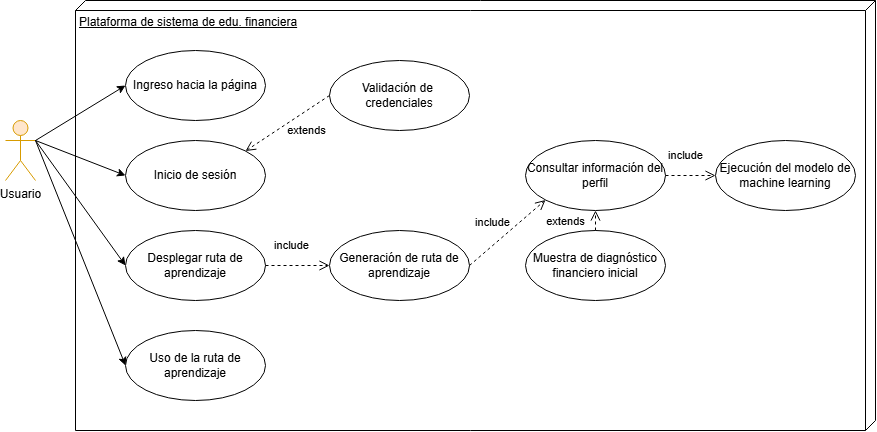
\includegraphics[width=12cm]{Imagenes/CasoUsoRF09.png}
	\caption[{Diagrama de caso de uso RF09.}]{\centering Diagrama de caso de uso RF09. \textit{Fuente:} Autores.}
	\label{fig:diagramacasousorf09}
\end{figure}

\subsubsection*{Vistas principales del prototipo}
\addcontentsline{toc}{subsubsection}{Vistas principales del prototipo}

Concorde a lo previamente descrito dentro de las historias de usuario y los casos de uso, se adjunta algunas vistas base del prototipo. Cabe aclarar que las siguientes ilustraciones para diseñar el modelo fueron obtenidas del sitio en el que esta ubicado el producto mínimo viable.

\begin{figure}[H]
	\centering
	\includegraphics[width=13cm]{Imagenes/EduFinanzasPP.png}
	\caption[{Vista principal.}]{\centering Vista principal. \textit{Fuente:} Autores.}
	\label{fig:vistaprincipal}
\end{figure}

\begin{figure}[H]
	\centering
	\includegraphics[width=13cm]{Imagenes/EduFinanzasPPF.png}
	\caption[{Vista de la página de progreso.}]{\centering Vista de la página de progreso. \textit{Fuente:} Autores.}
	\label{fig:vistaprogreso}
\end{figure}

\begin{figure}[H]
	\centering
	\includegraphics[width=13cm]{Imagenes/EduFinanzasPV.png}
	\caption[{Vista de la página de videoteca.}]{\centering Vista de la página de videoteca. \textit{Fuente:} Autores.}
	\label{fig:vistavideoteca}
\end{figure}